\subsection{Generating Geometry}

\subsubsection{Marching Cube Algorithm}
\begin{figure}[H]
  \centering
  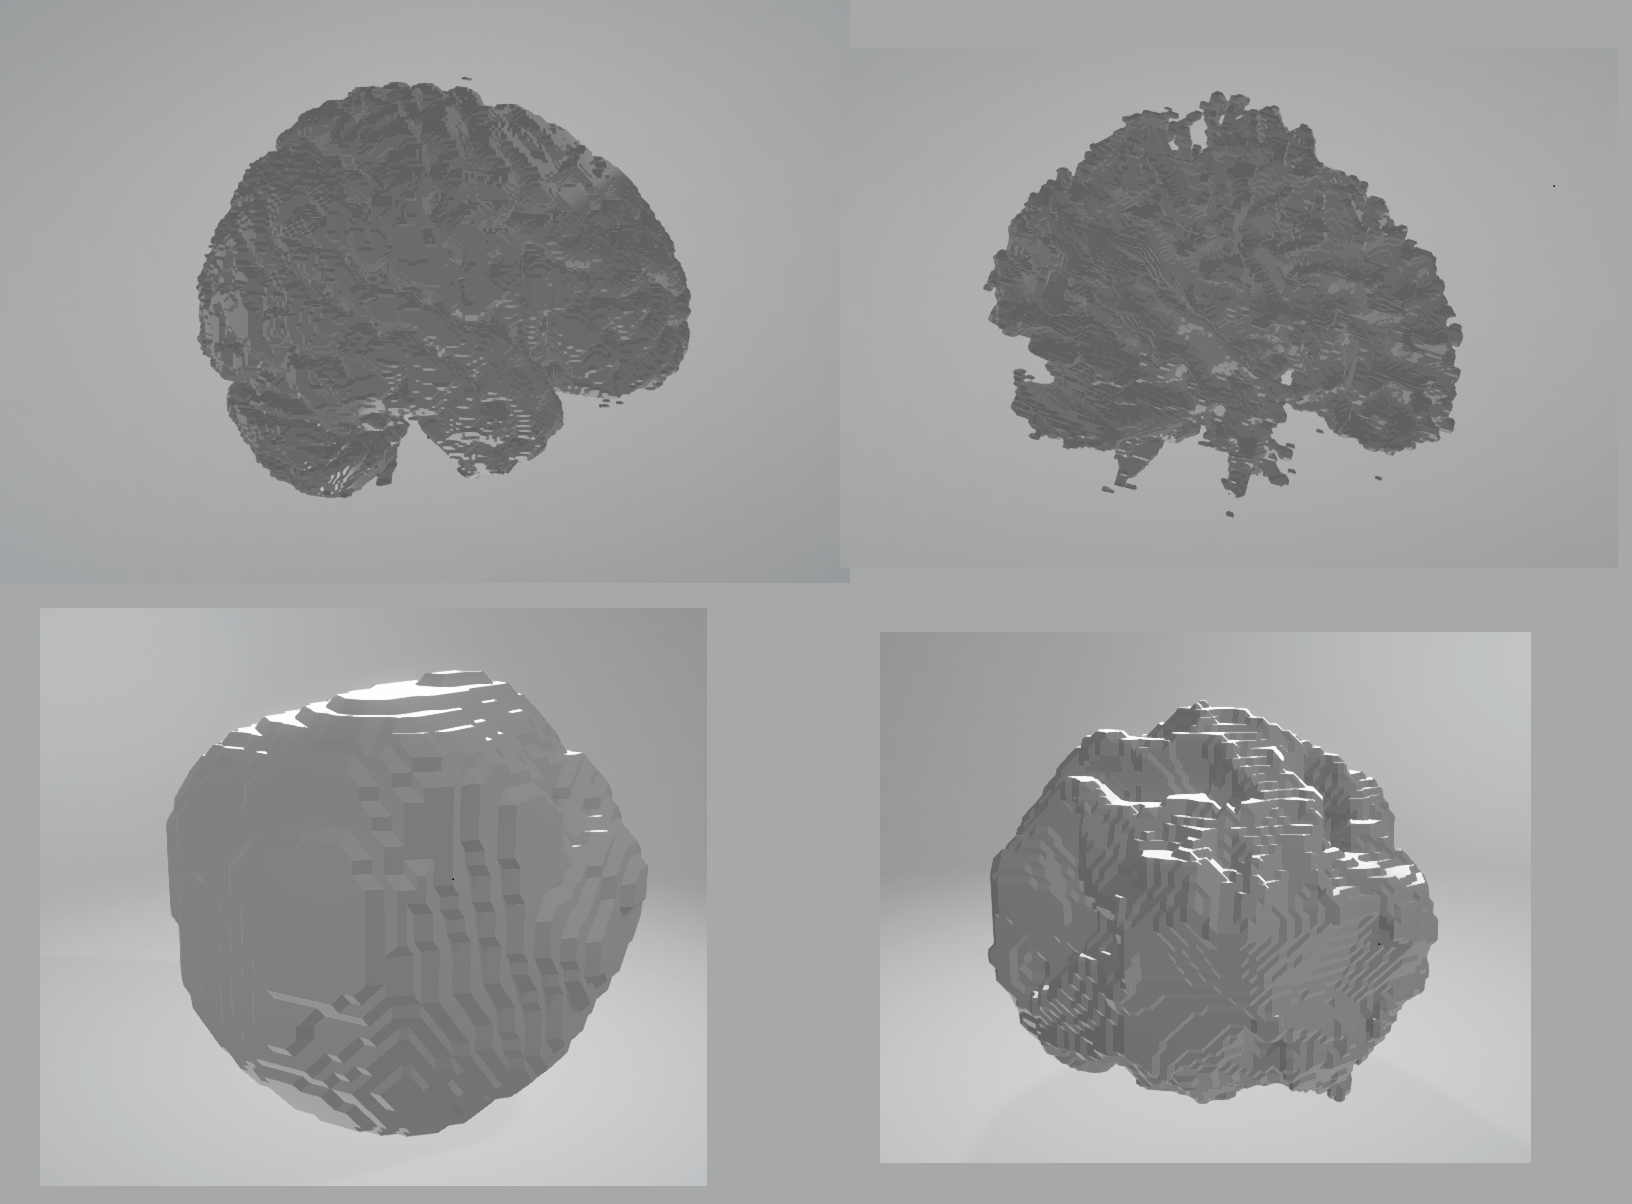
\includegraphics[width=\linewidth]{img/resultsMarchingCube.PNG}
  \caption{\textbf{Top Left:} Gray matter \textbf{Top Right:} White matter \textbf{Bottom Left:} Tumor \textbf{Bottom Right:} Abnormal tissue.}
  \label{fig:resultsMarchingCube}
\end{figure}

From a far it may seem that the models are what we expect but looking at the smaller object such as the tumor and the abnormal tissue it is clear that the resolution of the models are directly correlated with the number of slices within the DICOM file.  The marching cube algorithm generates these step wise artifacts which are the depth of the each slice within the MRI.  Because we can't use smoothing techniques, the only remedy to this is to increase the number of slices.  This will increase the computational cost and time to create a model for printing.  For most use cases we think that this is okay in the long run for holographic prints.  But for regular clinical practice like in the operating room or emergency care this is not feasible.  Nevertheless we prove that it is possible to perform semi-automatic segmentation in conjunction with marching cube algorithm to develop geometry.\\

All codes that generated this section can be found in Appendix \ref{sec:appendixPythonMain}.

\subsubsection{Volumetric Rendering Experiments}
As a foundation, the following steps cover the basics for creating a volumetric rendering of our MRI. After initiating these steps, attributes will be tested to determine rendering quality outputs, as needed, to remain as faithfully possible to the MRI aesthetic.\\

\paragraph{Step 1. DICOM Conversion}
Create batch conversion of DICOM to TIFF.\\

\paragraph{Step 2. Scene and Render Mode}
Open Blender (Blender Render mode): add a 1x1x1 cube to the scene, a spot light, and a point light, both lights with an intensity of 10.0.

\begin{figure}[H]
  \centering
  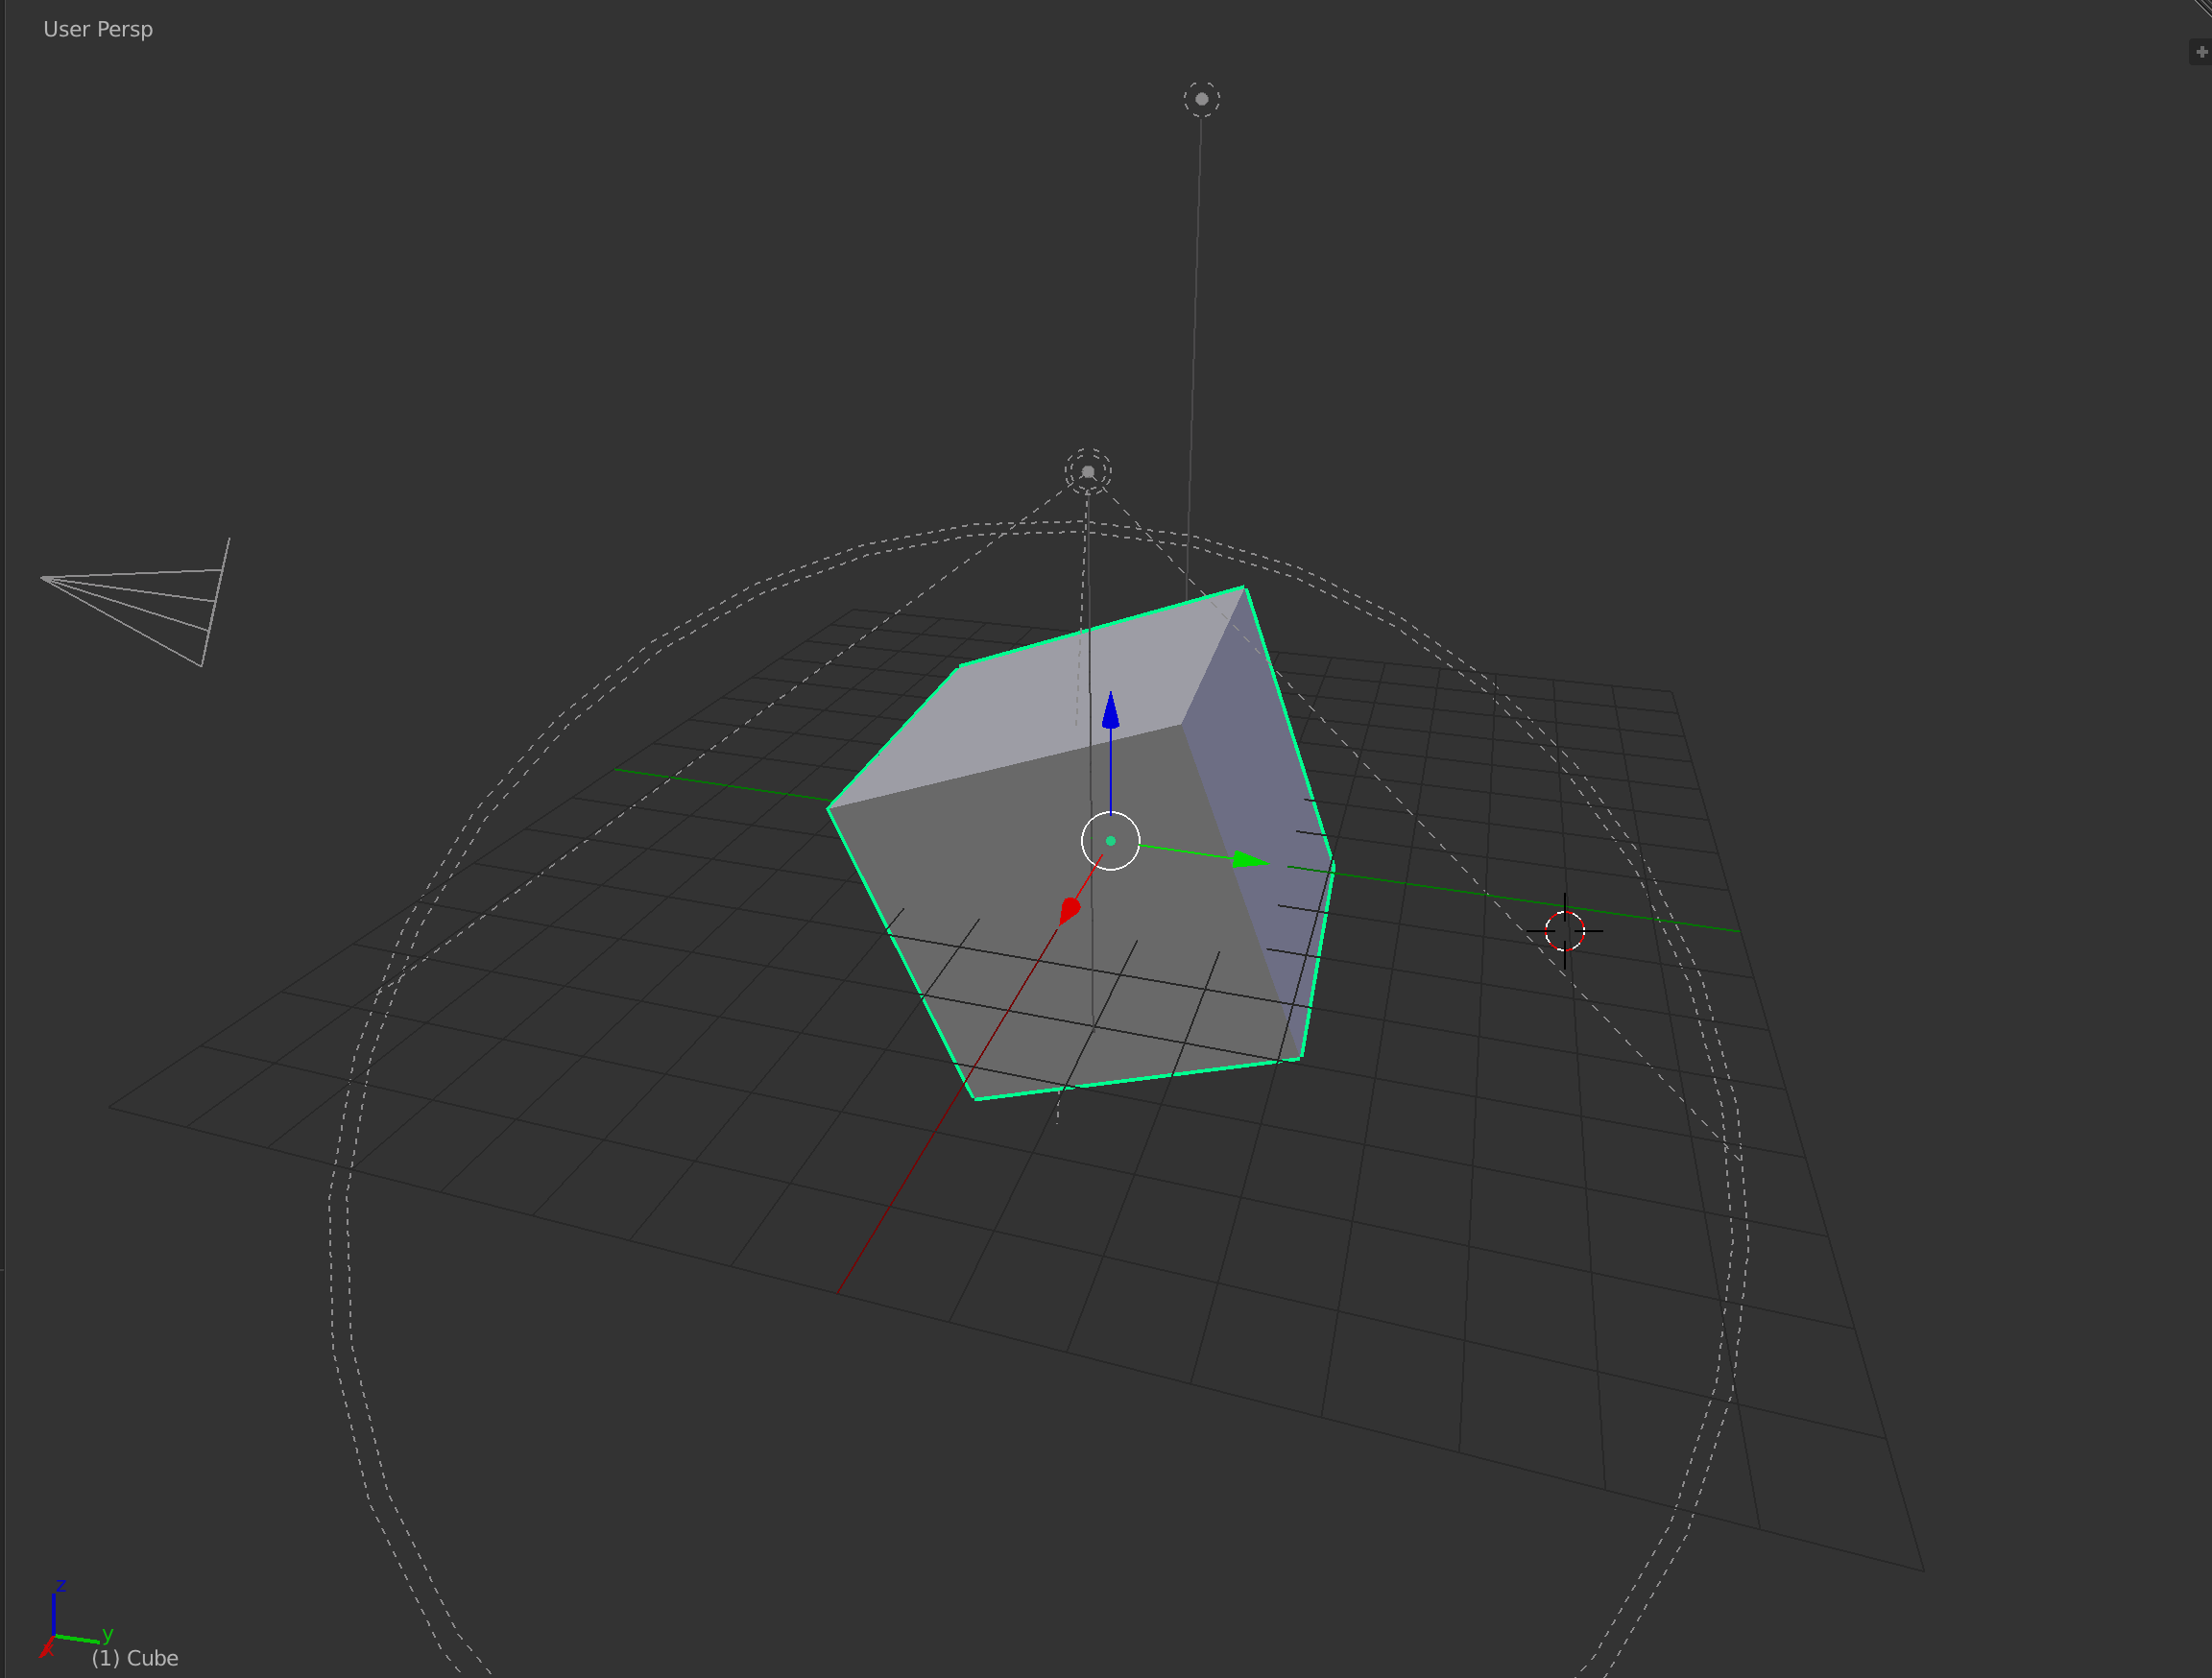
\includegraphics[width=0.5\linewidth]{img/cube.png}
  \label{fig:resultsCubeVolume}
\end{figure}

\paragraph{Step 3. Material Type}
Select cube and add a material node. Select ``Volume" for material type.
\begin{figure}[H]
  \centering
  
\includegraphics[width=0.5\linewidth]{img/volume.png}
  \label{fig:resultsCubeVolumeType}
\end{figure}


\paragraph{Step 4. Density and Integration}
Change the density value for the volume material to 0.0.
\begin{figure}[H]
  \centering
  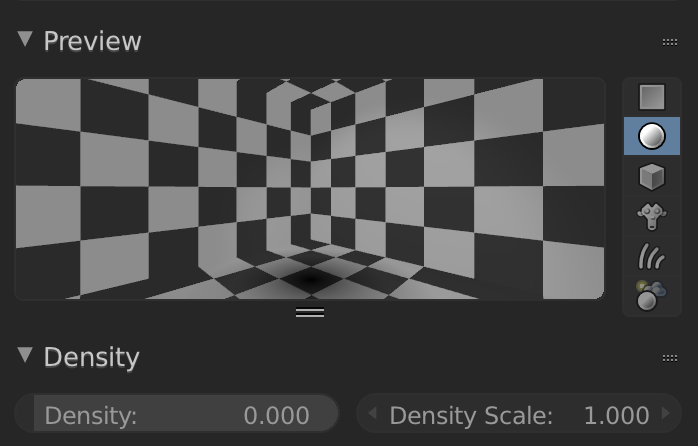
\includegraphics[width=0.5\linewidth]{img/density.png}
  \label{fig:resultsCubeDensity}
\end{figure}

Change integration step size to approx. 0.070.
\begin{figure}[H]
  \centering
  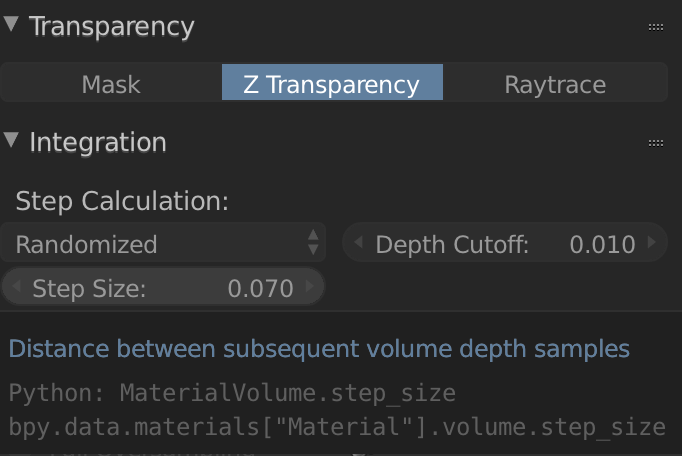
\includegraphics[width=0.5\linewidth]{img/integration.png}
  \label{fig:resultsCubeIntegration}
\end{figure}

\paragraph{Step 5. Voxel Data}
With cube still selected, add a texture node. Select ``Voxel Data" for texture type. Adjust texture brightness to approx. 0.800 and contrast to approx. 1.200. Adjust texture ramp for more control beyond brightness and contrast controls.
\begin{figure}[H]
  \centering
  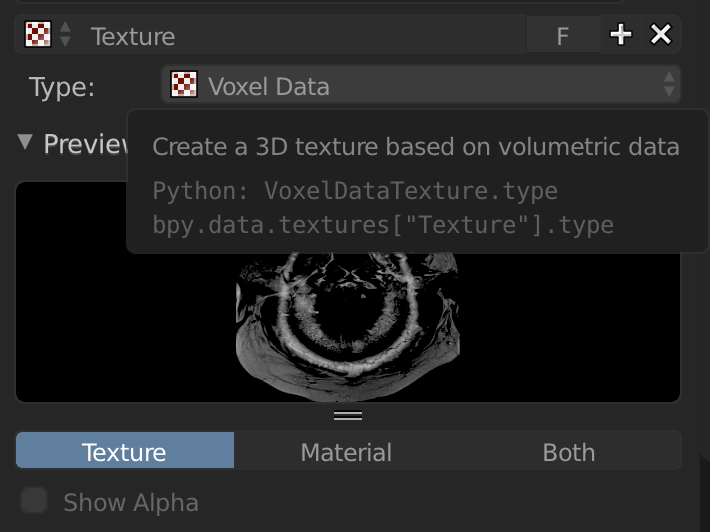
\includegraphics[width=0.5\linewidth]{img/voxel.png}
  \label{fig:resultsCubeVoxel}
\end{figure}

\paragraph{Volume Rendering Results}



\subsubsection{Jawa Method}